\documentclass[a4paper,10pt]{article}

% Hier die Nummer des Blatts und Autoren angeben.
\newcommand{\blatt}{11}
\newcommand{\autor}{Merlin Steuer, Till Schander, Lennart Bergmann}

\usepackage{hci}

\begin{document}
% Seitenkopf mit Informationen
\kopf
\renewcommand{\figurename}{Figure}

\aufgabe{16}

\subsection{Analyse}
Aufgrund der Kürze der Zeit haben wir uns dafür entschieden, nur ein kurzes Interview bestehend aus wenigen Fragen durchzuführen. Das Augenmerk sollte dabei auf der Login- und der Willkommensseite liegen. Als Zielgruppe wählten wir zunächst nur die Studierenden, da wir nur deren Ansicht kennen und somit verbessern können.

Die Fragen lauten:
\begin{enumerate}
\item Nutzt du OLAT in diesem Semester?
\item Wenn ja: Wieviele OLAT-Kurse belegst du dieses Semester?
\item Wie viele OLAT-Kurse hast du bereits belegt?
\item Kennst du die Informationen, welche neben dem LOGIN-Formular auf der OLAT-Login-Seite zu finden sind?
\item Wie wichtig sind diese Informationen für dich? (1 - 10)
\item Wie viele Kurse hast du in OLAT als Favoriten markiert?
\item Für welche Informationen besuchst du OLAT besonders häufig? Bewertungen, Übungsblätter, Skripte, Diskussionen, Zusatzmaterialien, Sonstige?
\item Wie effizient findest du die für dich wichtigen Funktionen in OLAT? (1 - 10)
\item Wie wichtig sind dir Neuigkeiten über bspw. Sicherheitslücken oder neue Features? (1 - 10)
\end{enumerate}

Die Antworten auf diese Fragen lauteten:
\begin{enumerate}
\item ja, ja, nein, ja, ja
\item 1, 2, -, 1, 1
\item 2, 1, 1, 2, 1
\item nein, nein, nein, nein, nein
\item 0, 0, 2, 4, 0
\item 0, 0, 1, 0, 0
\item \begin{itemize}
    \item Übungsblätter, Bewertungen
    \item Übungsblätter, Bewertungen
    \item Skript, Übungsblätter, Bewertungen
    \item Skript, Übungsblätter
    \item Übungsblätter
\end{itemize}
\item 4, 6, 5, 7, 3
\item 3, 6, 6, 7, 5
\end{enumerate}

Es ist also trotz der kleinen Testmenge zu betrachten, dass viele OLAT für Übungsblätter und Bewertungen jener aufsuchen, diese Informationen jedoch nicht sonderlich effizient auffinden.
Auch scheinen die Informationen neben dem Login-Formulat auf der Startseite in dieser Form überflüssig. Der Wunsch über Neuigkeiten informiert zu werden (insbesondere in Bezug auf Sicherheitslücken) ist jedoch gegeben.

\subsection{Design}

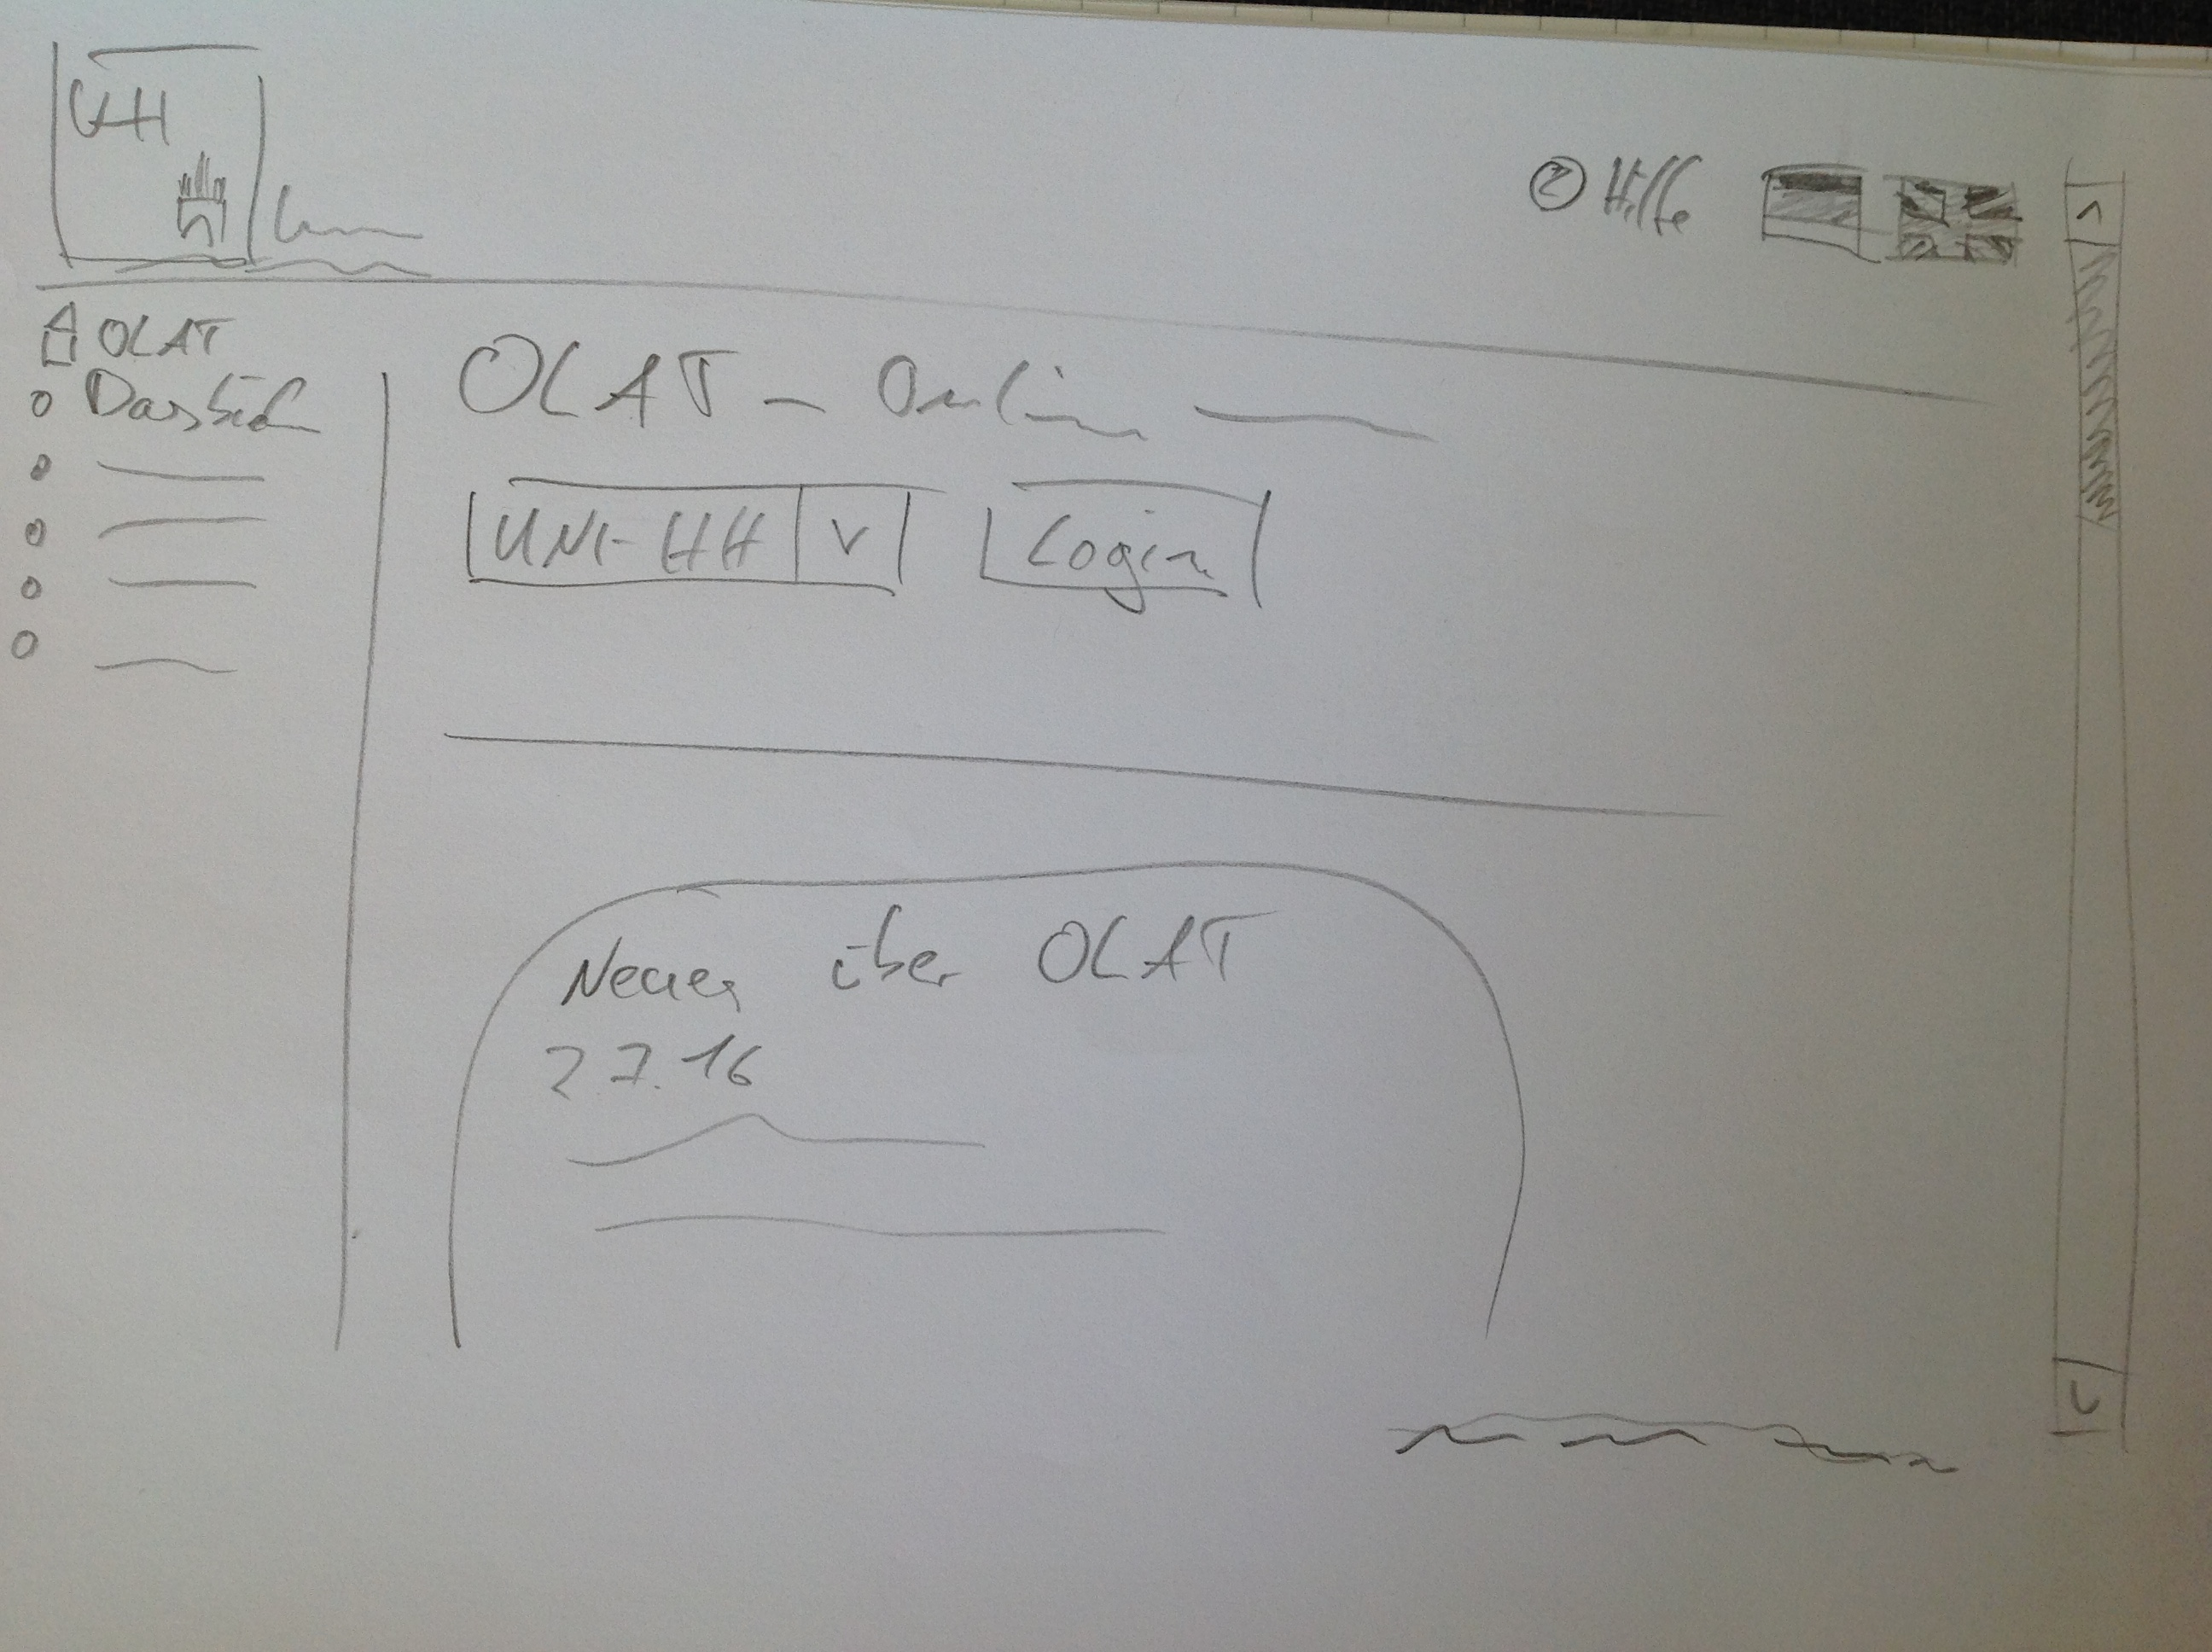
\includegraphics[scale=0.18]{images/IMG_0362.JPG}

Die Start-/Login-Seite wurde etwas entschlackt. Die Support-Emails kann man nun unter der Hilfe finden(Merging similiar options). Die Flaggen zur Sprachauswahl sind nun sofort beide sichtbar(exposing options), da ein Dropdown für zwei Optionen überflüssig ist. Das Hauptaugenmerk liegt auf dem Login, da die meisten User dafür die Seite besuchen.

Zudem haben wir uns entschieden den restlichen Platz für einen Newsstream zu nutzen, in dem wichtige Updates oder neue Features angekündigt werden können.


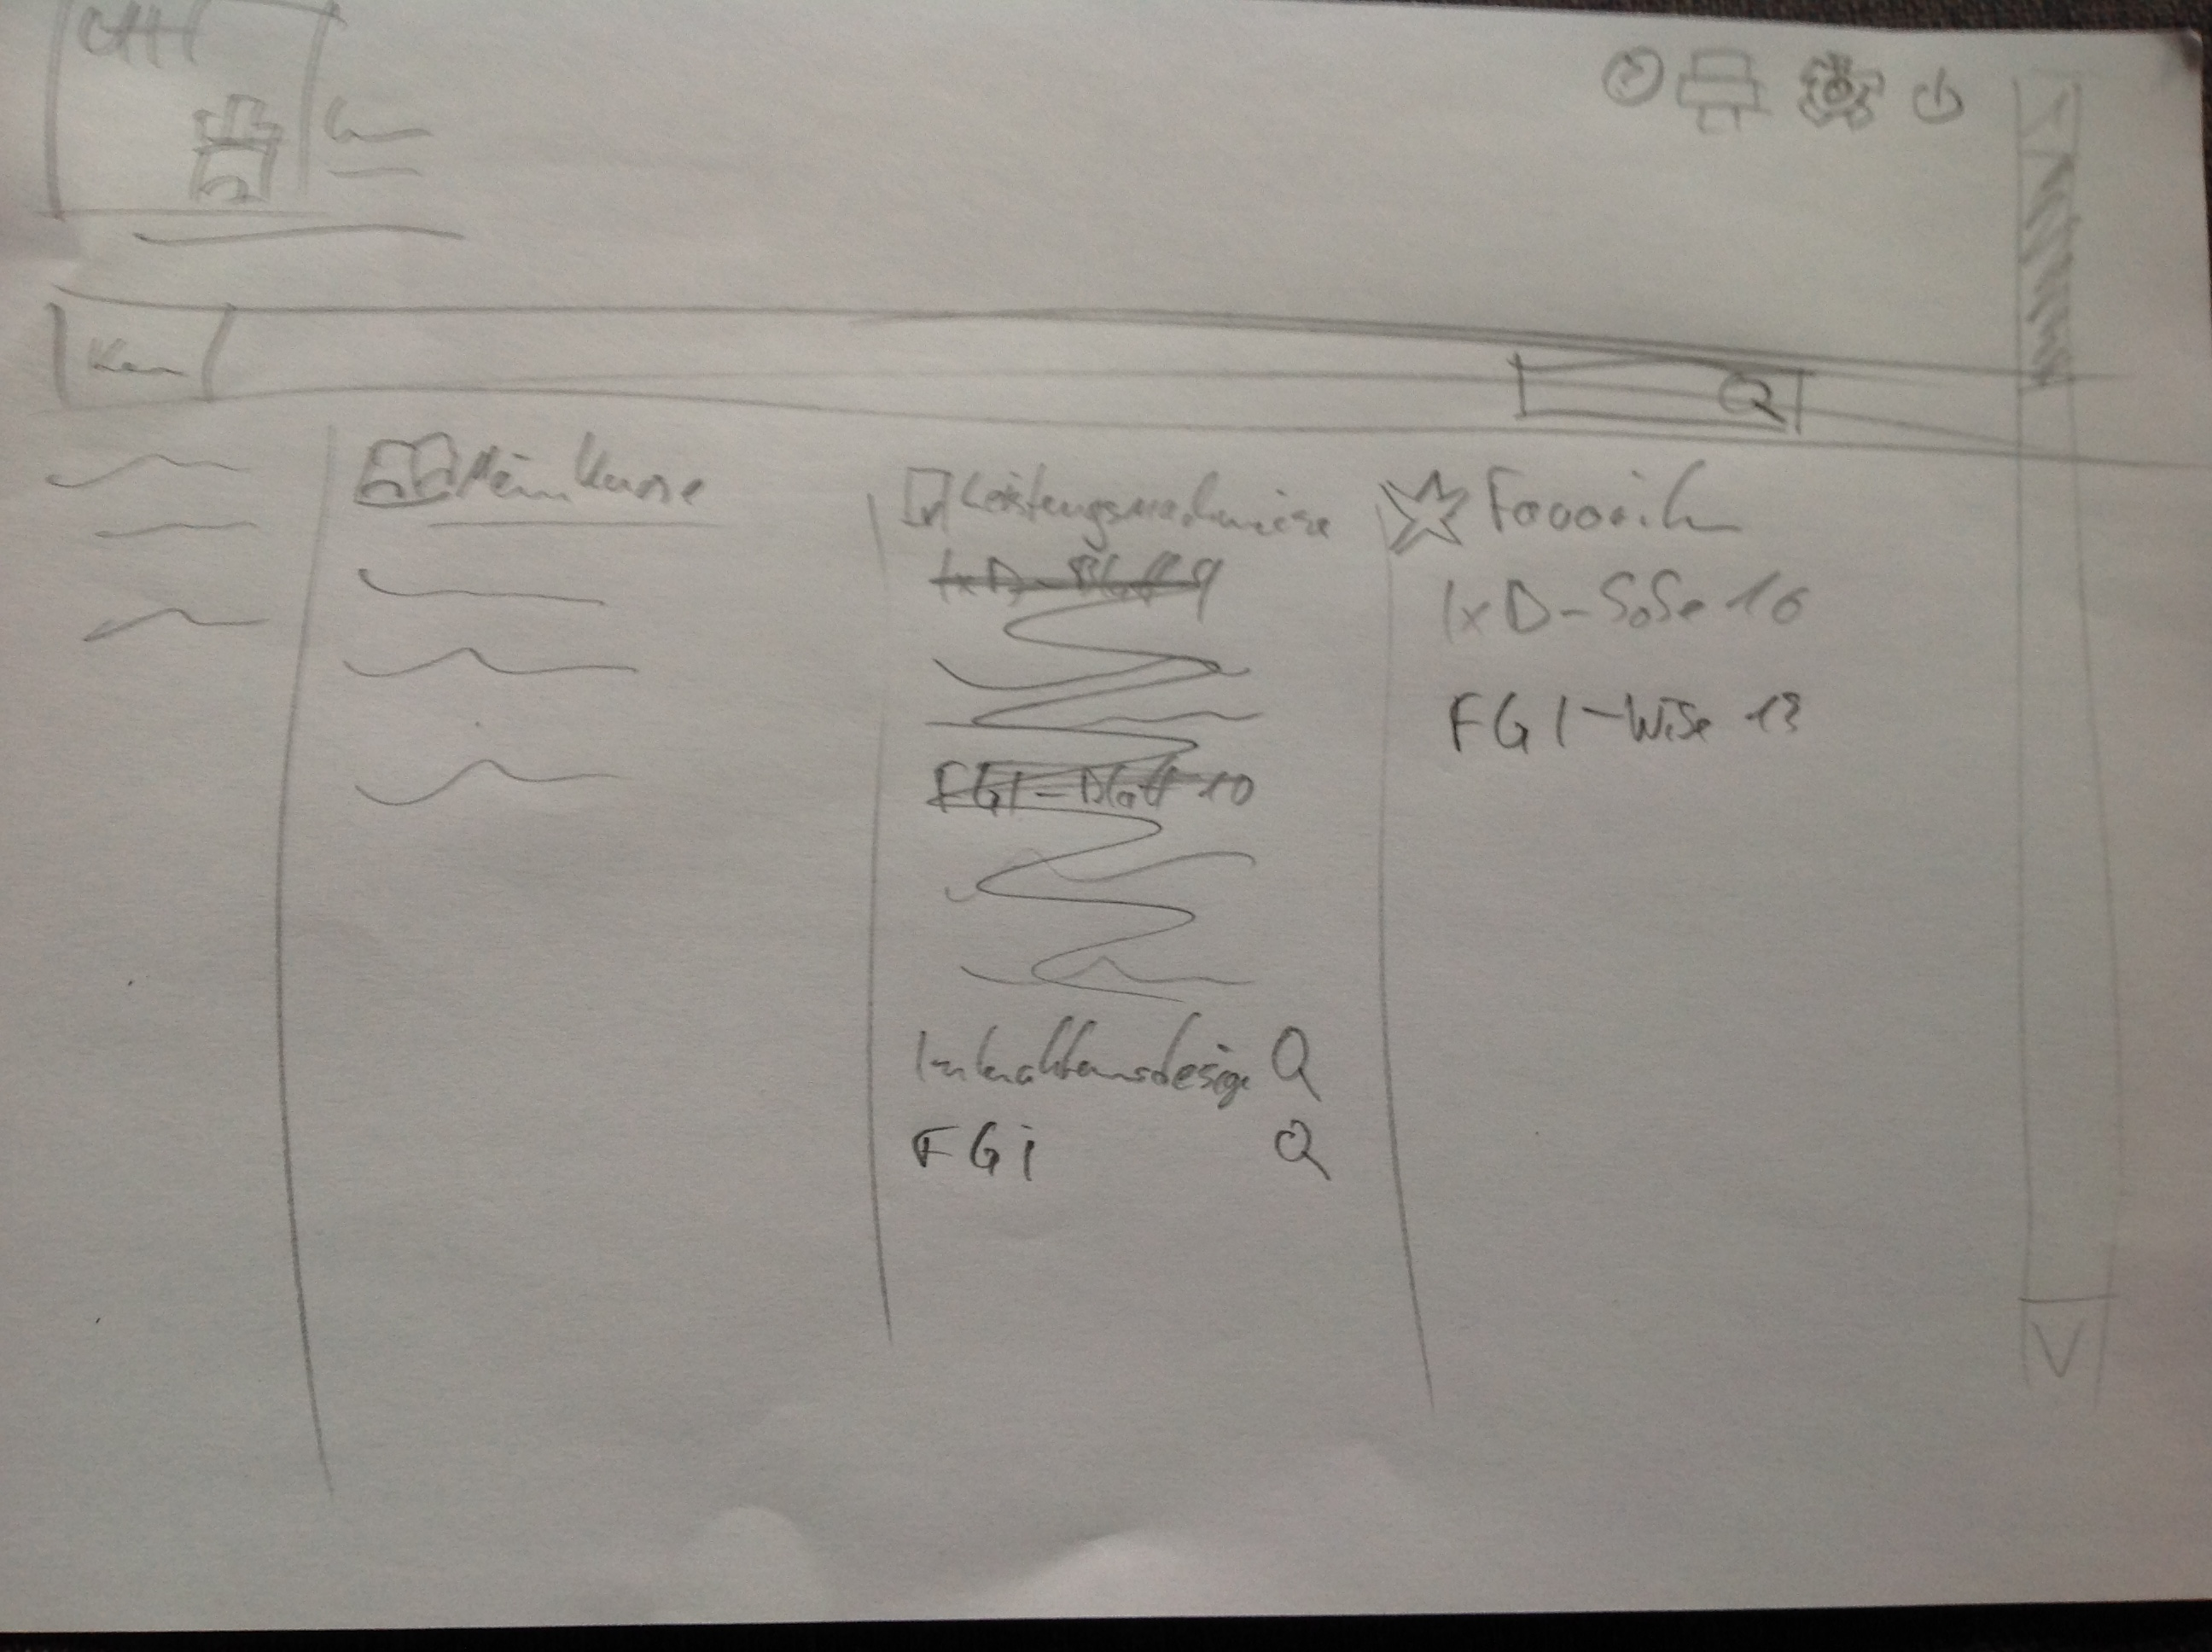
\includegraphics[scale=0.18]{images/IMG_0363.JPG}

Die Wilkommen-Seite wirkte sehr überladen. Wir haben sie etwas aufgeräumt und uns beim re-design auf die wichtigsten Aspekte beschränkt, auch wenn das Dashboard erhalten bleibt. Die meisten User werden OLAT aufrufen um in ihre Kurse zu gucken, oder ihre Bewertungen einzusehen, weshalb wir hierfür einen "Clear Entry Point" geschaffen haben. Die Zeile für "Many Workspaces" bleibt natürlich erhalten, wird aber nur noch für geöffnete Kurse benutzt. Das Hauptaugenmerk liegt darauf, dem Nutzer einen simplere, eingängigere Oberfläche zu präsentieren.

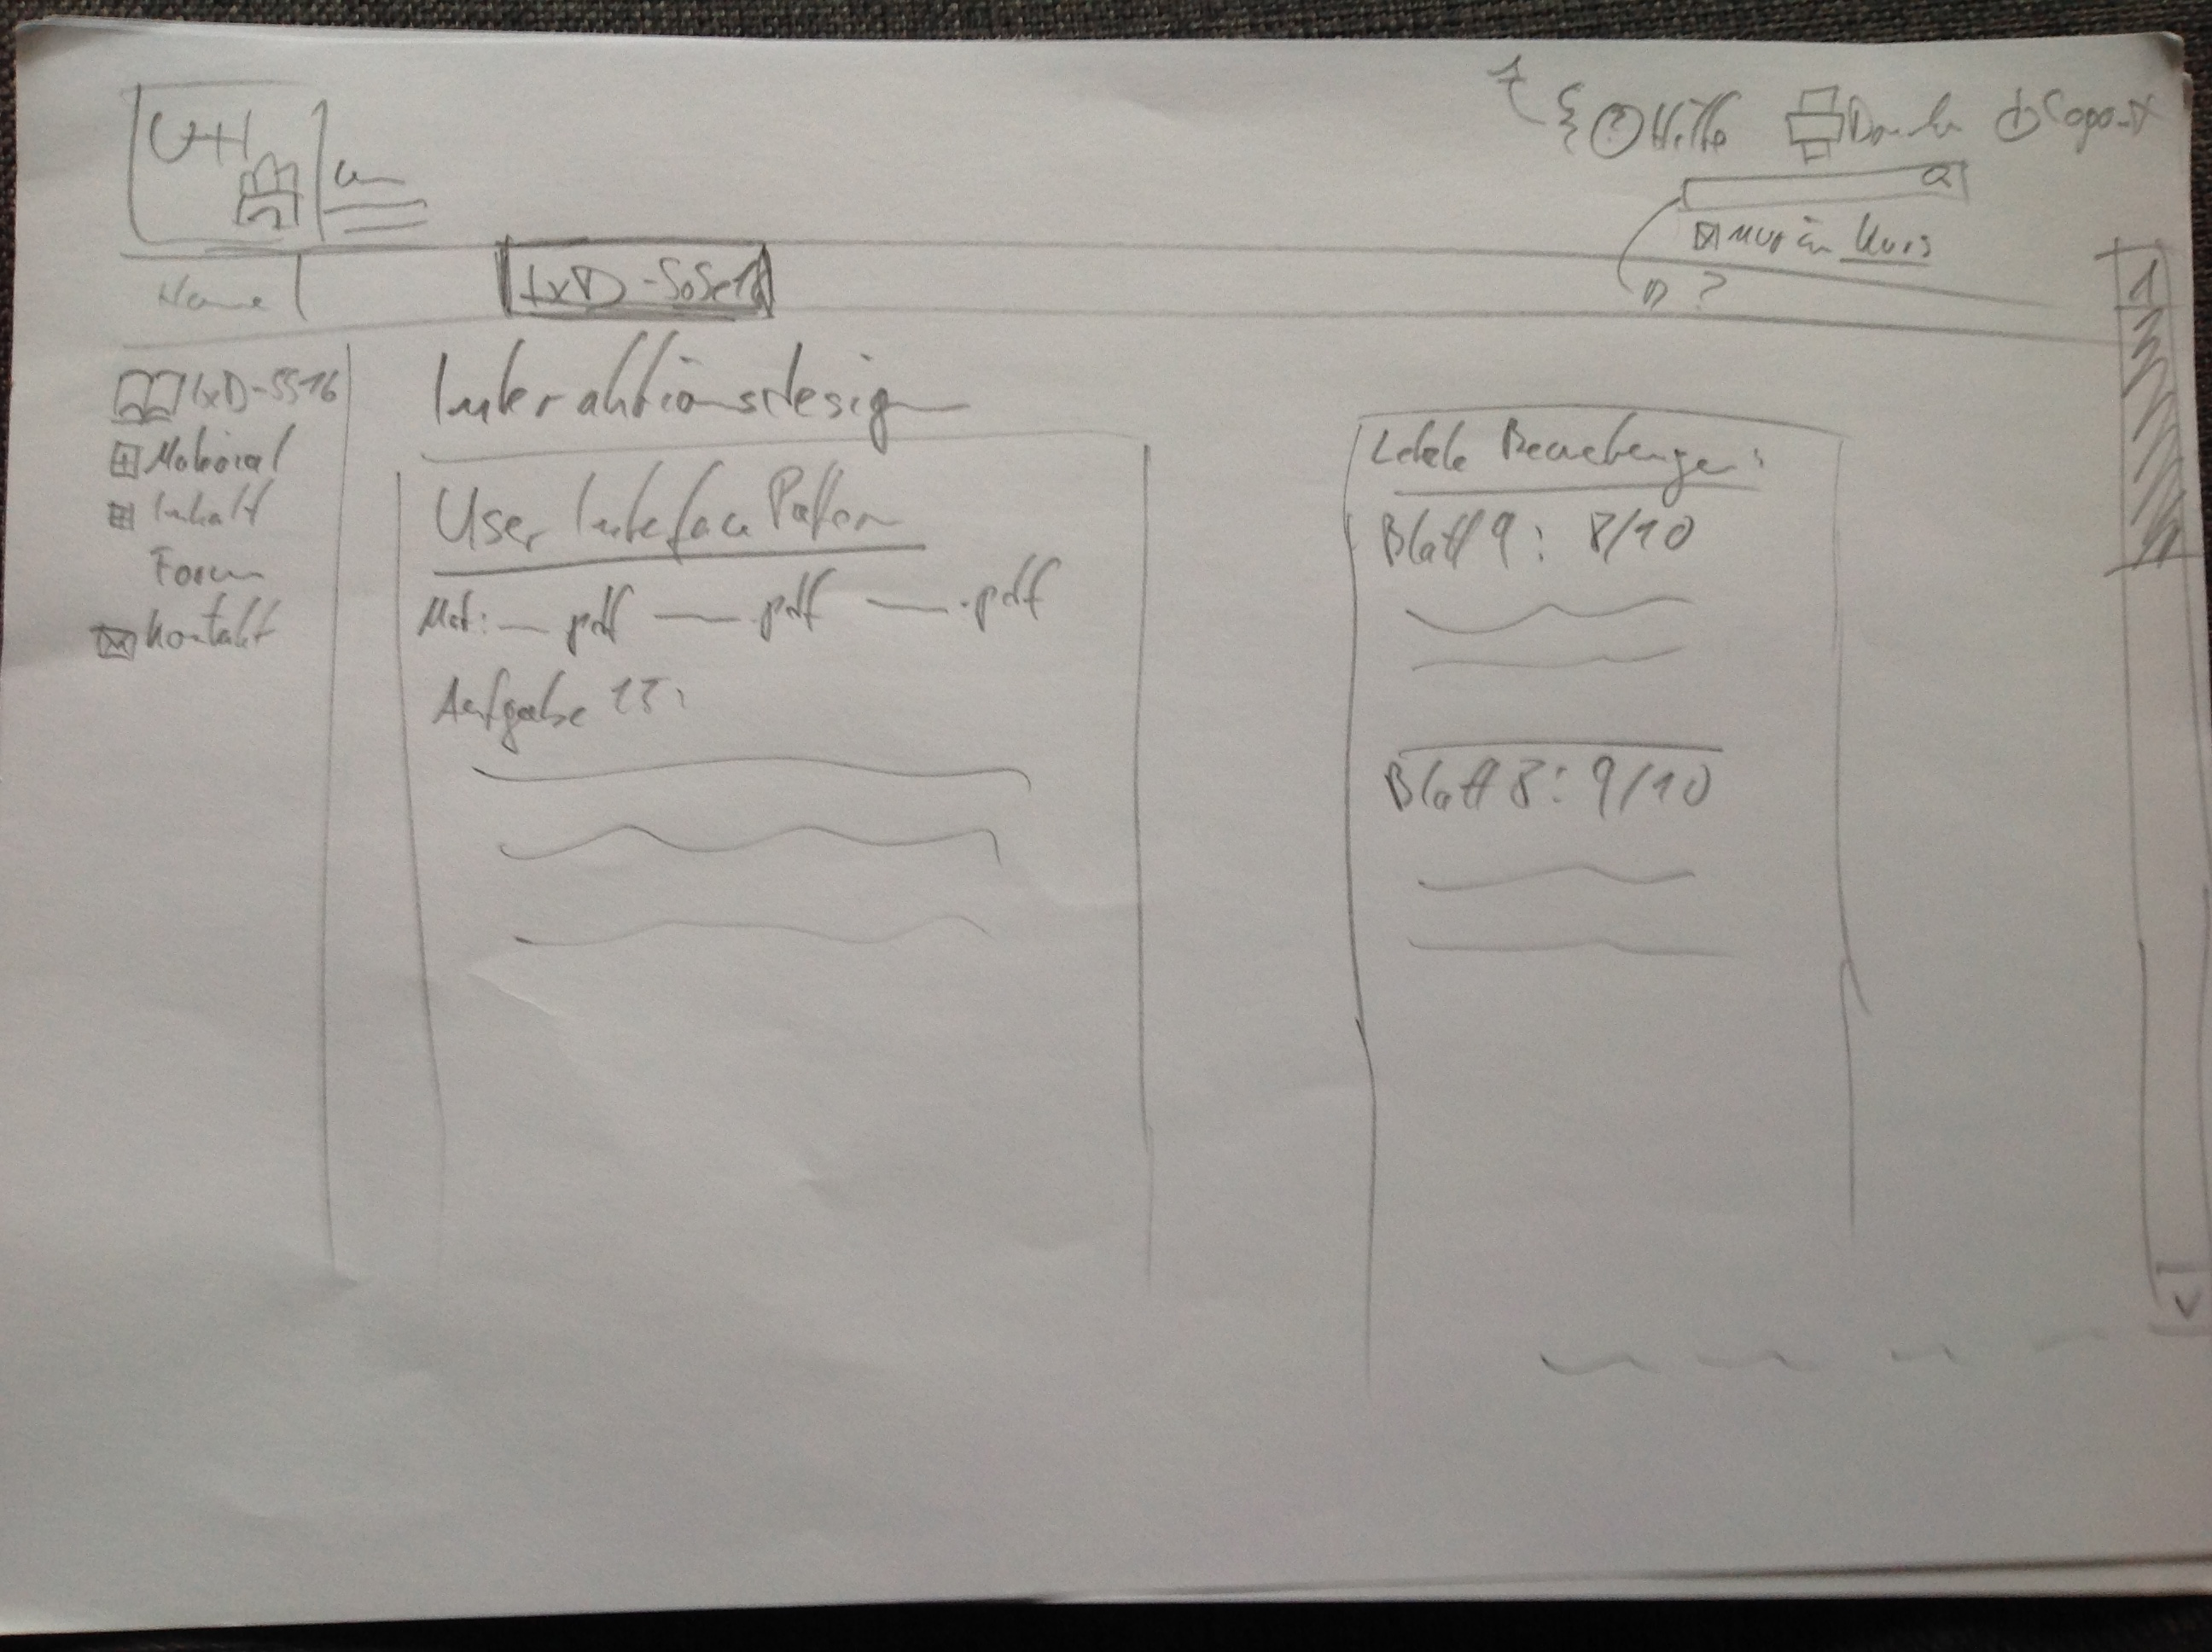
\includegraphics[scale=0.18]{images/IMG_0364.JPG}

Auch hier haben wir etwas aufgeräumt. Es gibt nun schon auf der Startseite einen Überblick über die neusten Inhalte (Newsstream) sowie die letzten Bewertungen, da die meisten User diese Dinge am ehesten sehen wollen. Die bekannten Seiten bleiben natürlich erhalten(Alternative Views). Der "Ordner" heißt jetzt "Material", damit der User weiß, was ihn hier erwartet. Auch wurden das Wiki, die Linkliste und das Literaturverzeichnis hierhin verschoben, um das Menü zu vereinfachen und zusammengehörige Optionen zu gruppieren. Zur besseren Verständichkeit heißt "Inhalt" jetzt "Kursinhalt" und "Email" wurde zu "Kontakt". Feature/Search/Browse.

Alle Bereiche haben oben links den Escape Hatch, und teilweise zusätzlich noch den Home-Button. 

\subsection{Implementierung} 
Willkommen:

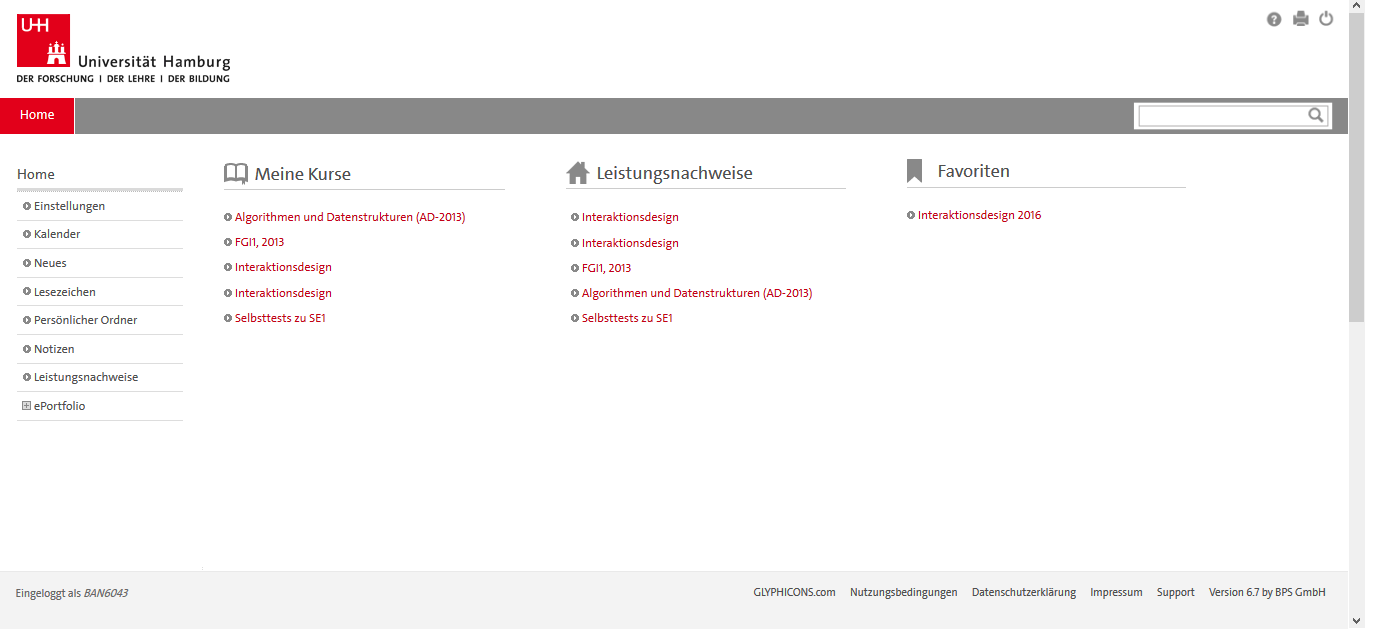
\includegraphics[scale=0.4]{images/wilkommen_seite.png}

Login:

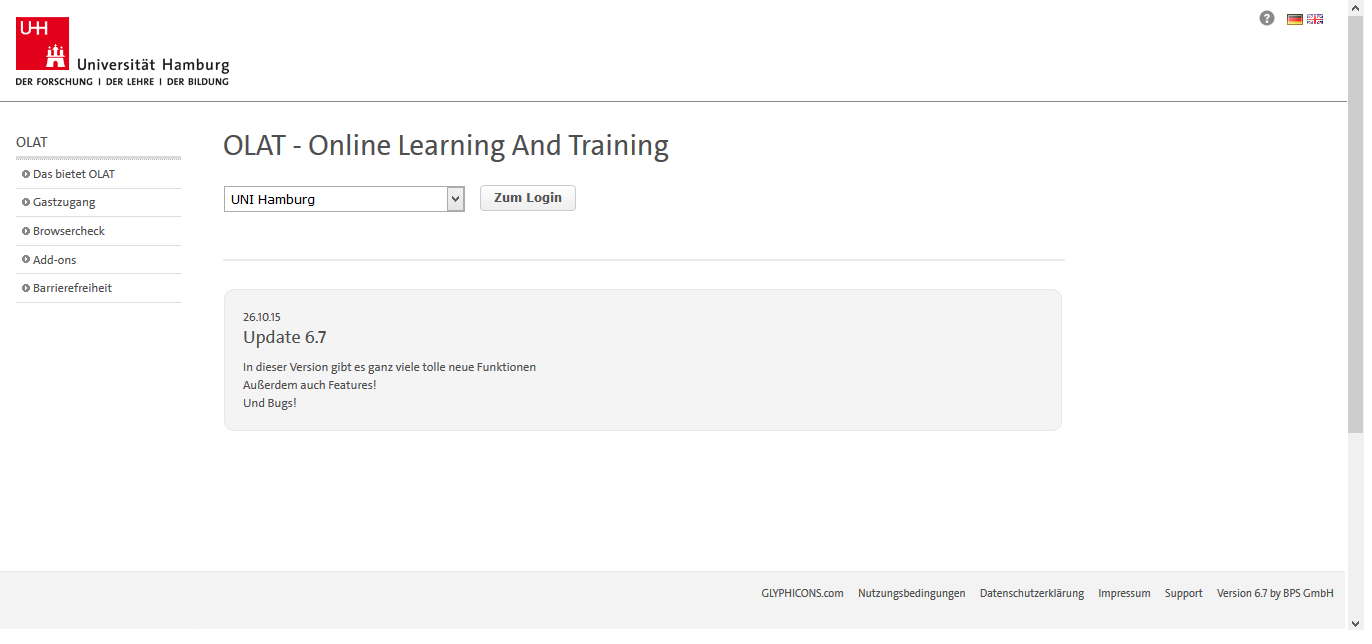
\includegraphics[scale=0.4]{images/login_seite.png}

Kurs:

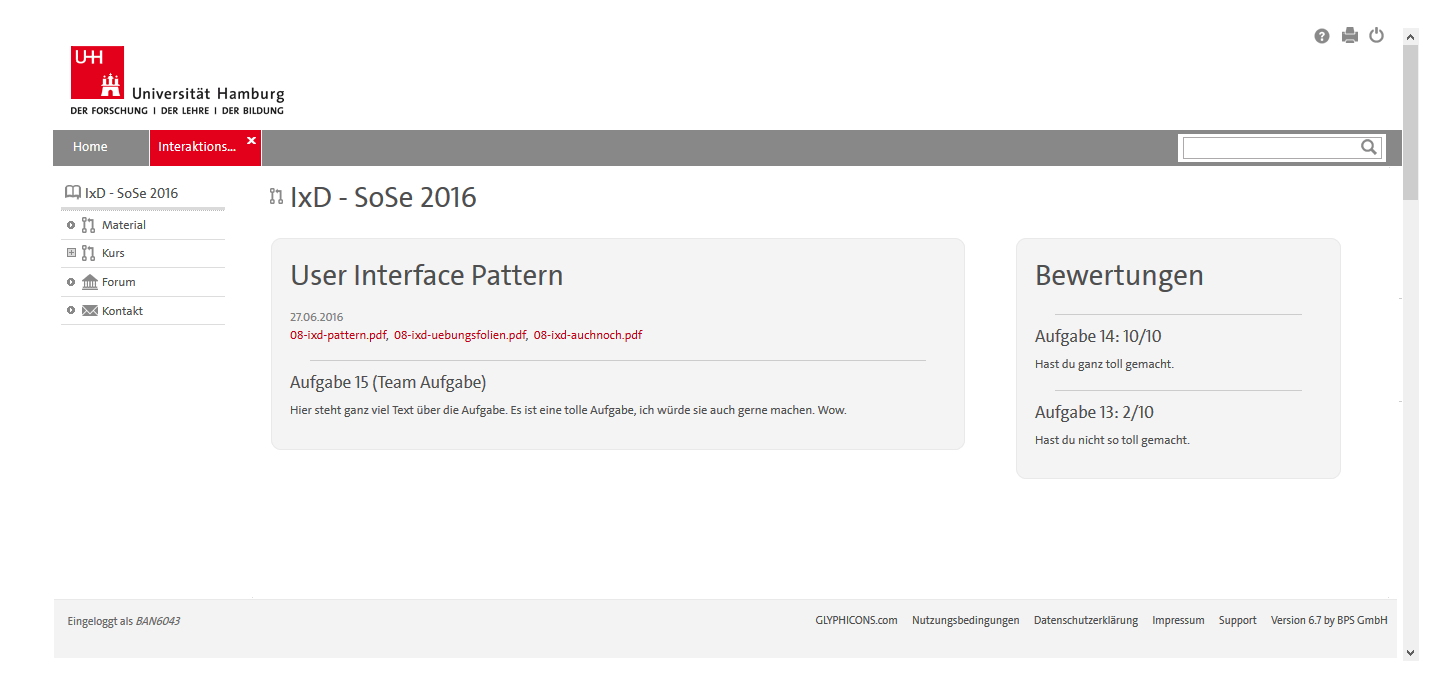
\includegraphics[scale=0.4]{images/ixd_seite.png}
\end{document}
